\documentclass[a4paper,11pt]{article}

\title{Solutions to unfolding distributions}
\author{ACM}
\date{\today}

\usepackage{placeins}
\usepackage{amsmath,amssymb,amsfonts}
\usepackage{graphicx}
\usepackage{amsmath}

%%%  Draft
\newcommand{\fixme}[1]{ \mbox{\bf{FIXME:} \it{#1}} } 

\begin{document}
\maketitle

\section{Understanding unfolding}

The Unfolded spectra can be found using, eg, RooUnfold:
\begin{verbatim}
ROOT.gSystem.Load("${HOME}/Downloads/RooUnfold-1.1.1/libRooUnfold.so")
##  prepare the response matrix
# assume a flat prior
R = ROOT.RooUnfoldResponse(None,None,resp)
u = ROOT.RooUnfoldInvert(R,reco)
u.SetName("unfolder1")
h = u.Hreco(ROOT.RooUnfold.kNone) ##  error propagation down with toys
h.SetName("unfold")

u2 = ROOT.RooUnfoldInvert(R,reco_fluct)
u2.SetName("unfolder2")
u2.SetNToys(1000)
h2 = u2.Hreco( ROOT.RooUnfold.kCovToy)
h2.SetName("unfold2")

\end{verbatim}

The result is shown in figure~\ref{fig:sol1}: the unfolded distribution with no-fluctuations should be by-construction identical to the one used for generating it; 
small differences may be due to the numeric precision of the floating point representation inside a computer, that act as a fluctuation smearing. 
The one that had fluctuations inside, nevertheless is the maximum-likelihood (ML) estimator and therefore the best linear unbiased estimator (BLUE), has a very huge variance.
\fixme{Need to give them an error if we use gaus ones}

\begin{figure}[H]
	\centering
	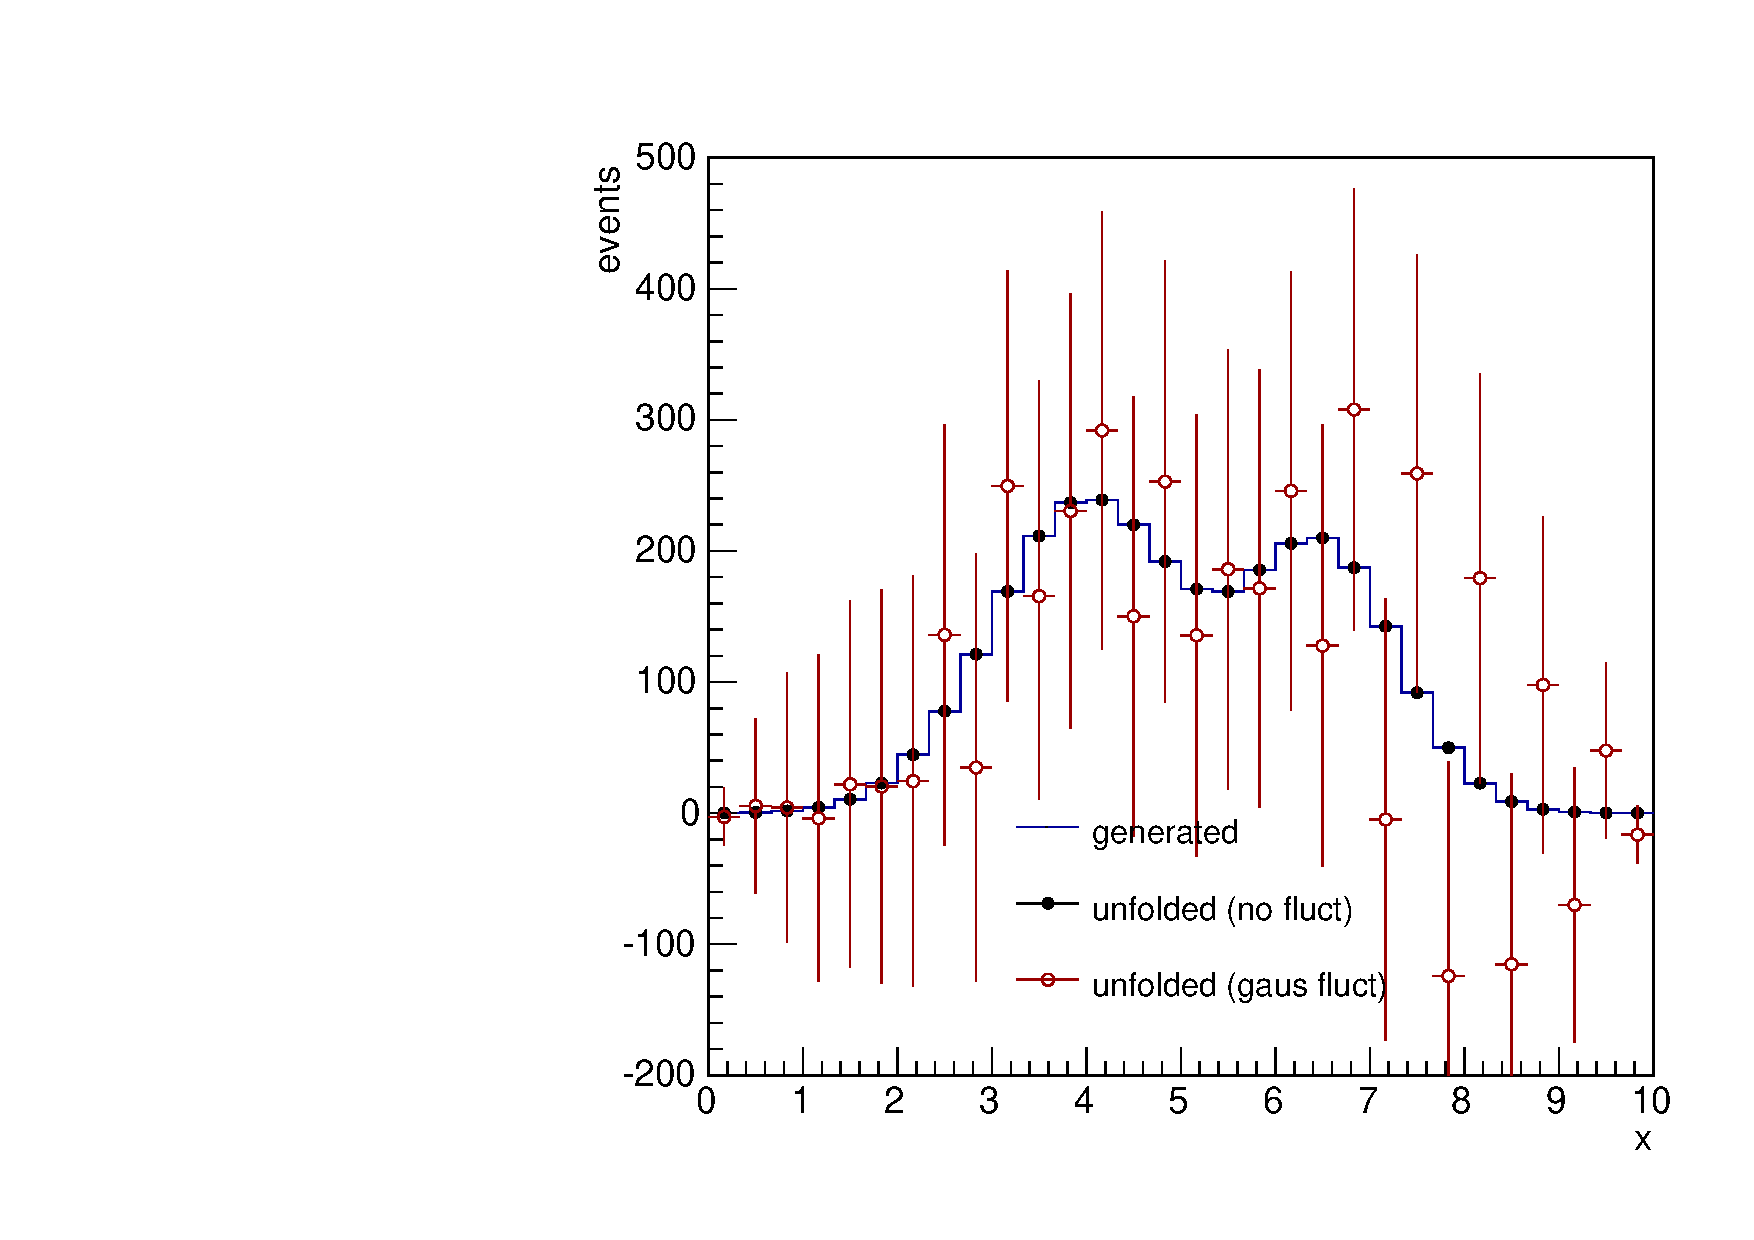
\includegraphics[width=0.618\textwidth]{figs/gen-unfold.pdf}
	\caption{ \label{fig:sol1} The two unfolded distribution compared with the one used to generate them.}
\end{figure}

\FloatBarrier
\end{document}
